% Chapter 3 - Results 

\chapter{Numerical experiments} % Main chapter title

\label{chap:results} % For referencing the chapter elsewhere, use \ref{Chapter1} 

\lhead{Chapter 3. \emph{Comparison of methods}} % This is for the header on each page - perhaps a shortened title

%----------------------------------------------------------------------------------------
\section{General results}
Using least-squares assures a SPD system which is an important advantage over regular Galerkin. On the downside the matrix obtained from least-squares is a lot worse conditioned and complex to create. For second order equations the LS-system created by transforming the PDE to a set of hyperbolic equations (as done in this project) is three times as big as when solving it directly. Comparing the correctness of the solution to the problems
%as done in for example figure~\ref{fig:ConvergencePoisson} shows that the convergence rate is the same as for Galerkin, but with a finite element basis the value of the residual is slightly higher for the least-squares method, and for spectral basis functions least-squares converge to a higher residual.
reveals that the error of the least-squares solution converges to a slightly higher value. This effect can be explained by the functional that is minimized. Notice that in the least-squares methods you minimize the \textbf{square} of the residual, while with Galerkin you do not square your residual. Since the correctness of both methods are restricted by the smoothness of the solution and the number of nodes used to discretize the domain, LS-methods will minimize the residual squared down to a given precision and hence the residual itself will end up on a slightly higher value. 
%\newpage
%
\subsection{Poisson problem}
The test case is constructed by choosing the loading function and analytical solution as 
\begin{align}
	f(x,y) &=  e^{x}(\pi^2-1)\sin(\pi y)\\
	u(x,y) &=  e^{x}\sin(\pi y). % Analytical solution
	\label{eq:poissonTestCasevariables}
\end{align}
%
The corresponding Poisson equation is then solved by imposing the Dirichlet boundary condition $g$ such that $g(\partial \Omega) = u(\partial \Omega)$.
In figure\eref{fig:ConvergencePoisson} the convergence in $L^{\infty}$ is plotted. Note that in the finite element case the basis functions used, do not fulfill the necessary conditions as explained in chapter \ref{finite element}. The least-squares solution is therefore notably less accurate. Using a spectral basis the least-squares solution seems to converge at the same rate, but to a higher residual. The condition number as a function of the number of basis functions is plotted in figure\eref{fig:ConditionPoisson}. The loglog plot shows that the slope is twice as steep for least-squares than for Galerkin indicating the relation 
%
\begin{align}
	\kappa(A^{LS})=C\kappa(A^{G})^{2}.
	\label{eq:condNumber}
\end{align}
%
Where $A^{LS}$ and $A^{G}$ denotes the stiffness matrices for each method and $C$ is some positive constant. 
 This result is as expected from the discussion in \ref{condNum}.   
%
\begin{figure}[t]
  \centering
  \begin{subfigure}[b]{0.48\textwidth}
	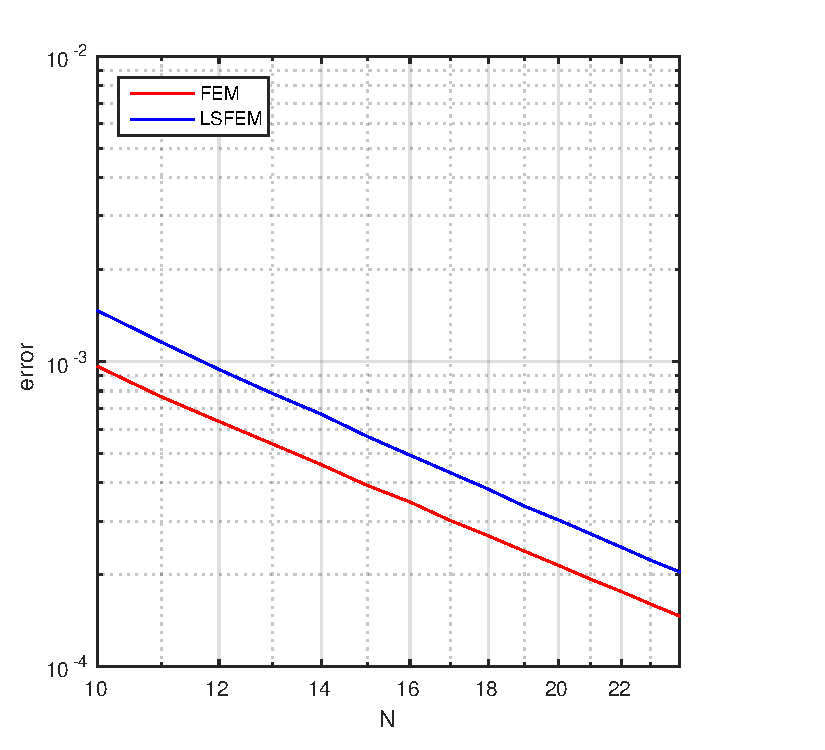
\includegraphics[width=\textwidth]{Figures/errorFEM-LSFEM.pdf}
  \end{subfigure}%
  \quad
  \begin{subfigure}[b]{0.48\textwidth}
	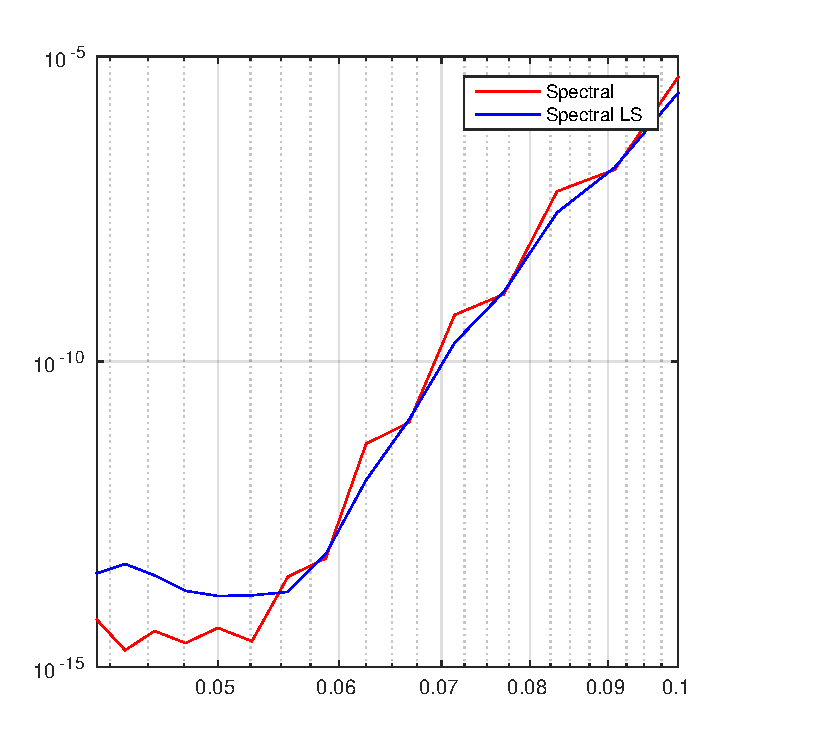
\includegraphics[width=\textwidth]{Figures/errorSpec-SpecLS.pdf}
  \end{subfigure}
          %(or a blank line to force the subfigure onto a new line)
  \vspace{-0.1\baselineskip}
  \caption{Convergence of Galerkin and corresponding least-squares formulation on the Poisson problem.}
  \label{fig:ConvergencePoisson}
\end{figure}
%
\begin{figure}[ht]
  \centering
  %\begin{subfigure}[b]{0.48\textwidth}
	%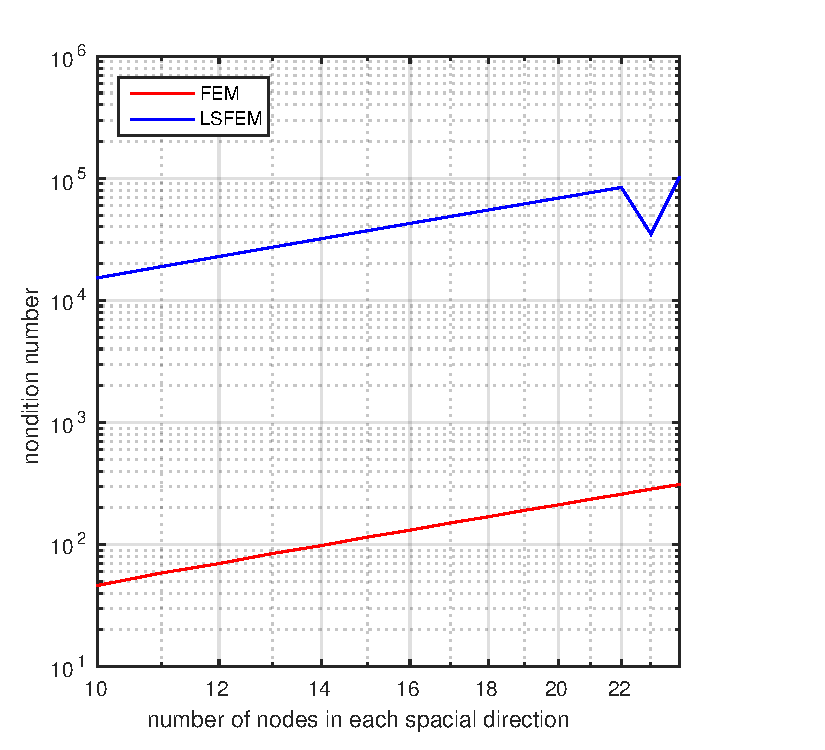
\includegraphics[width=\textwidth]{Figures/condFEM-LSFEM.pdf}
  %\end{subfigure}%
  %\quad
  %\begin{subfigure}[b]{0.48\textwidth}
	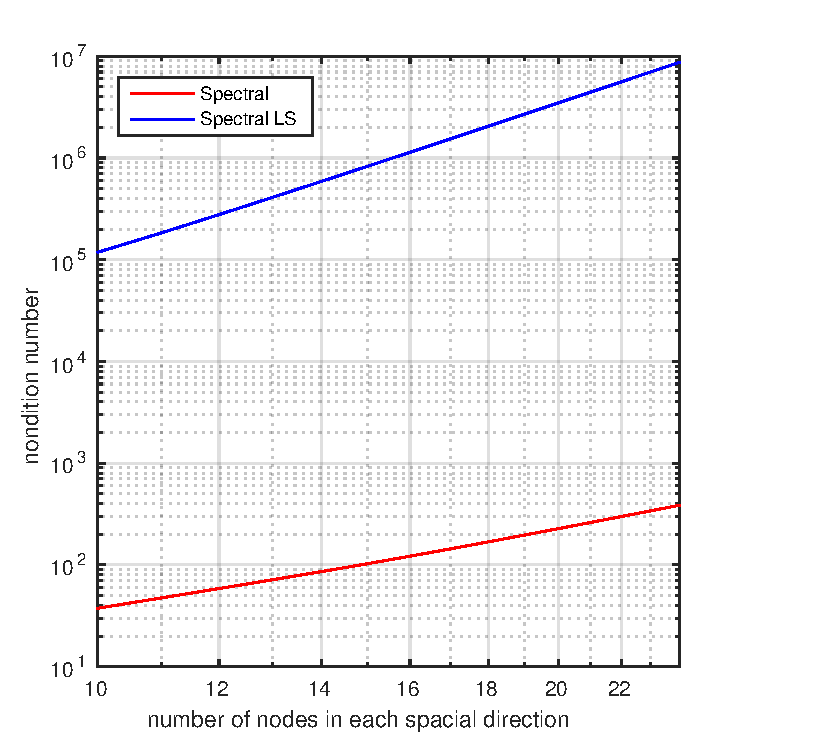
\includegraphics[width=0.6\textwidth]{Figures/condSpec-SpecLS.pdf}
  %\end{subfigure}
          %(or a blank line to force the subfigure onto a new line)
  %\vspace{-0.1\baselineskip}
  \caption{Condition number of Galerkin and least-squares formulation on the Poisson problem.}
  \label{fig:ConditionPoisson}
\end{figure}
%
\subsection{Diffusion transport problem}
For this problem all results presented are obtained with spectral basis functions. It is experimented with different ways of implementing the boundary conditions, both Dirichlet and Neumann conditions are implemented using both methods described in section \ref{BC}.
Let us start by letting $\mathbf{b} = [b_1(x),b_2(y)] $ be a normalized (in $L^{\infty}$ sense) vector field, and $\mu,b \in \mathbb{R}$ be the scalars used to scale the diffusion and convection term. The equation analysed is then written as 
\begin{align}
	-\mu \Delta u + b \; (\mathbf{b} \cdot \nabla u) = f .
	\label{eq:difftransForConditionNumberPlotting}
\end{align}
%
\begin{figure}[h!]
  \centering
  \begin{subfigure}[b]{0.48\textwidth}
		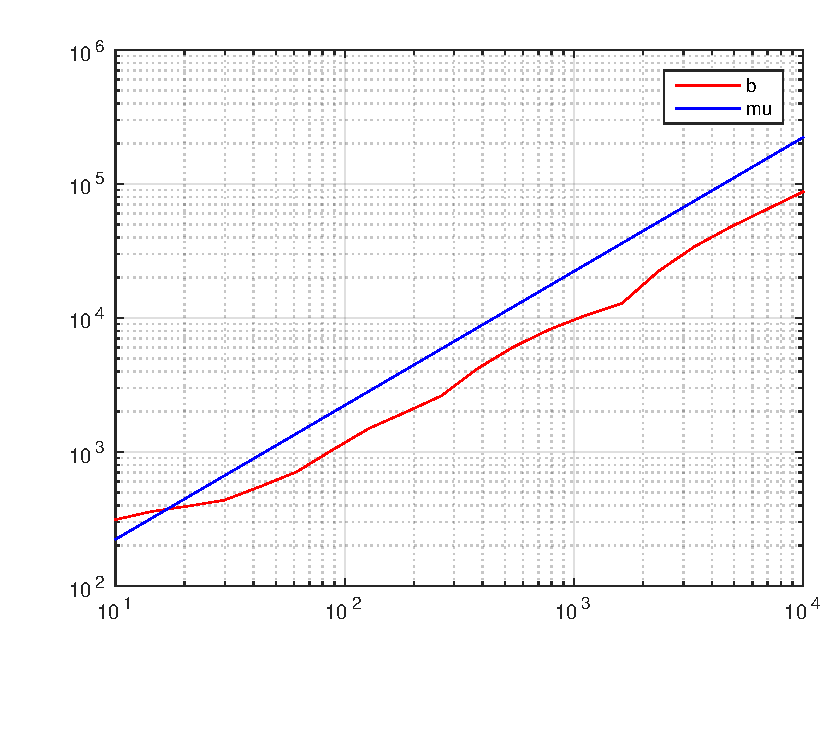
\includegraphics[width=\textwidth]{Figures/Spec_difftrans_ConditionNumber.pdf}
  \end{subfigure}%
  \quad
  \begin{subfigure}[b]{0.48\textwidth}
		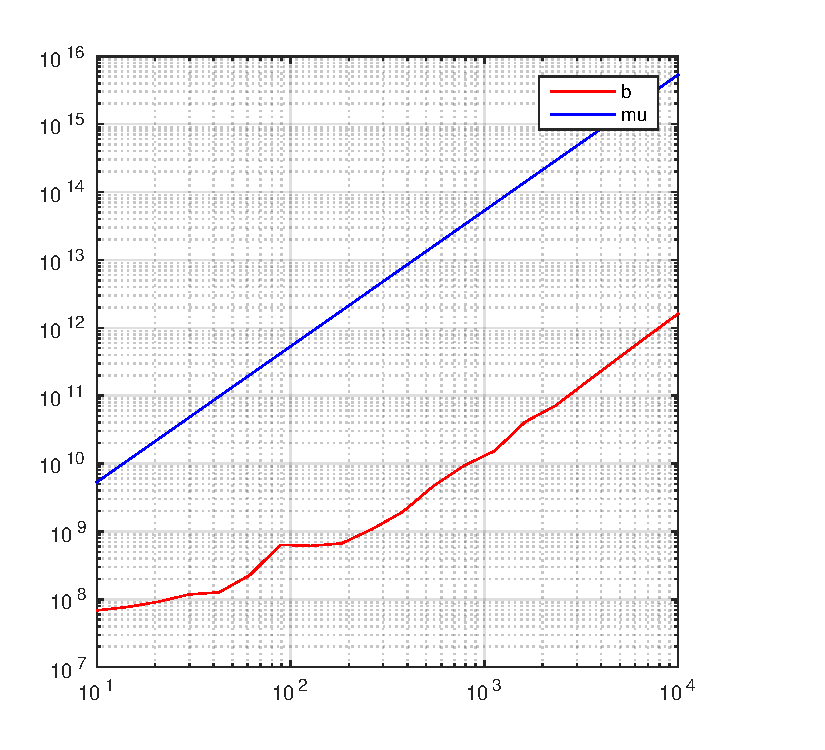
\includegraphics[width=\textwidth]{Figures/Spec-LS_difftrans_ConditionNumber.pdf}
  \end{subfigure}
  \begin{subfigure}[b]{0.48\textwidth}
		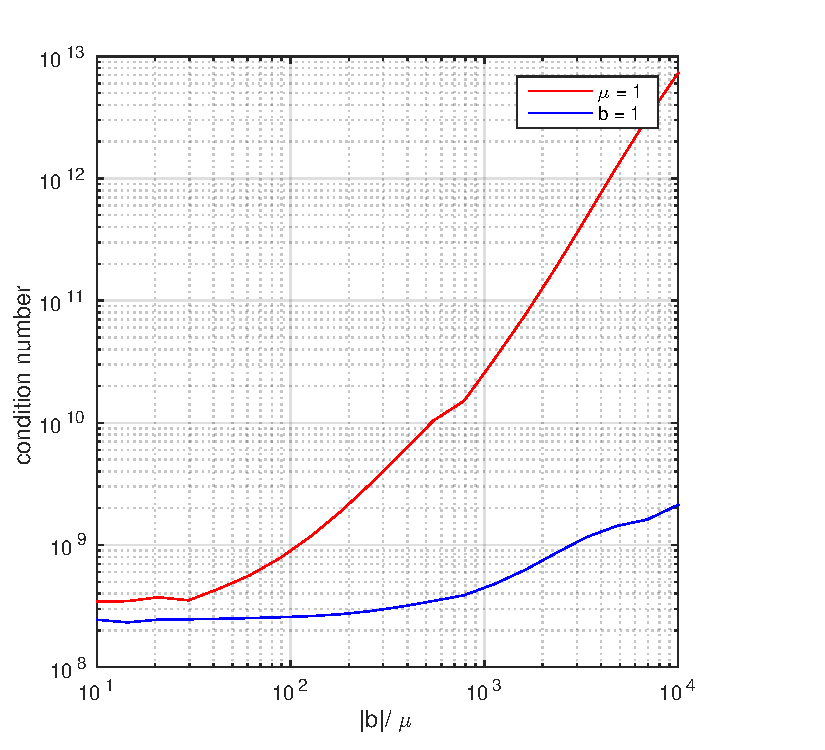
\includegraphics[width=\textwidth]{Figures/Spec-LS_difftrans_ConditionNumber_DirFunc.pdf}
  \end{subfigure}
          %(or a blank line to force the subfigure onto a new line)
  \vspace{-0.1\baselineskip}
	\caption{plot of the condition number as a function of $|b|/\mu \sim \mathbb{P}e$ where $\mathbb{P}e$ is the Peclet number. The parameters $\mu$ and $b$ are varied in turns, $N=20,\mathbf{b} = -[x,y]$. In the upper left plot standard Galerkin is used, in the upper right I have implemented a least-squares formulation with boundary conditions implemented directly into the search space. Finally in the lower plot least-squares is used with the BCs added in the functional.}
  \label{fig:CondDifftransSpec}
\end{figure}
%
In figure\eref{fig:CondDifftransSpec} the condition number is analysed as a function of the relation between the parameters $\mu,b$. With the number of nodes $N$ held constant this is proportional to the Peclet number $\mathbb{P}e \sim |b|/\mu$ \cite{Quarteroni}. Notice that along the blue lines $\mu$ is decreasing and $b$ is held constant, while along the red lines $\mu$ is held constant and $b$ is decreasing. The plots reveal that for the least-squares case the condition number is significantly more dependent on large $b$ than on small $\mu$. Studying the construction of the matrices in chapter \ref{Specmets} it seems that blowing up $b$ the four terms in the $G^{LS}$-matrix will be extremely large in comparison with the last five elements of the total matrix. Making $\mu$ smaller will have a similar inverse effect to the $A^{LS}$-matrix, but the rest of the elements will work as counterweights making the total matrix better balanced hence also better conditioned. The way of implementing the boundary conditions also makes a difference. Clearly imposing the BCs directly in the basis is much better than adding the extra term to the functional.    

The convergence results are presented in figure\eref{fig:ConvergenceDifftransSpec} and the same results as for the Poisson problem are obtained. It is also clear that imposing the boundary conditions as a restriction in our search space is far more efficient than adding them as an extra term to the functional. 

%
\begin{figure}[h!]
  \centering
  \begin{subfigure}[b]{0.48\textwidth}
		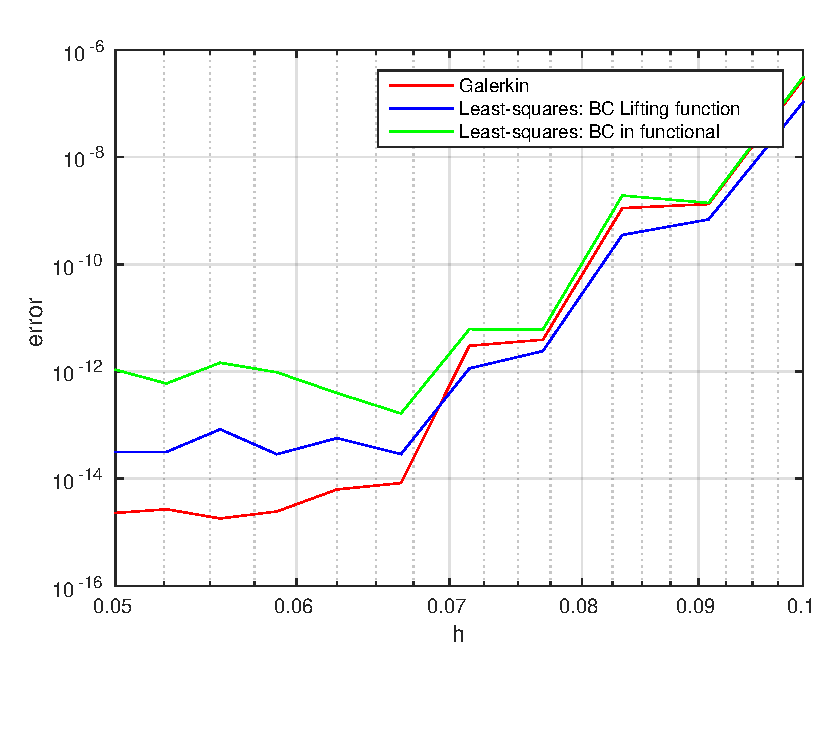
\includegraphics[width=\textwidth]{Figures/Spec_difftrans_Convergence.pdf}
  \end{subfigure}%
  \quad
  \begin{subfigure}[b]{0.48\textwidth}
		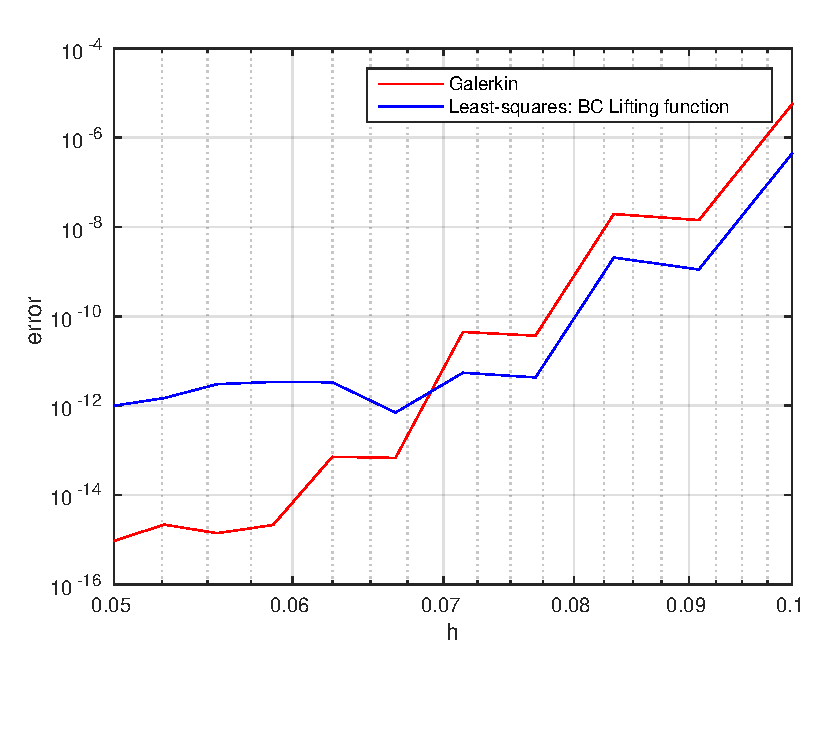
\includegraphics[width=\textwidth]{Figures/Spec_difftrans_Convergence_Neu.pdf}
  \end{subfigure}
          %(or a blank line to force the subfigure onto a new line)
  \vspace{-0.1\baselineskip}
	\caption{convergence plot of the diffusion transport test case with spectral basis functions and pure Dirichlet boundary conditions to the left and Neumann to the right  $b = 1,\mathbf{b} = -[x,y]$.}
  \label{fig:ConvergenceDifftransSpec}
\end{figure}
%

\newpage
\subsection{Diffusion transport equation surface plots}
%
\begin{figure}[h]
  \centering
  \begin{subfigure}[b]{0.48\textwidth}
	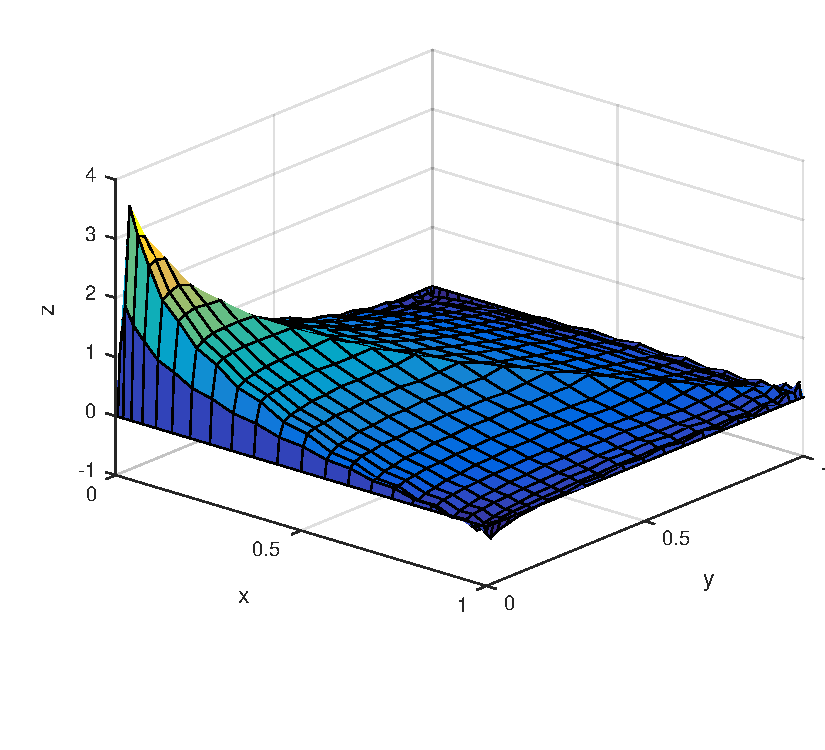
\includegraphics[width=\textwidth]{Figures/Spec_difftrans_aNeg.pdf}
  \end{subfigure}%
  \quad
  \begin{subfigure}[b]{0.48\textwidth}
	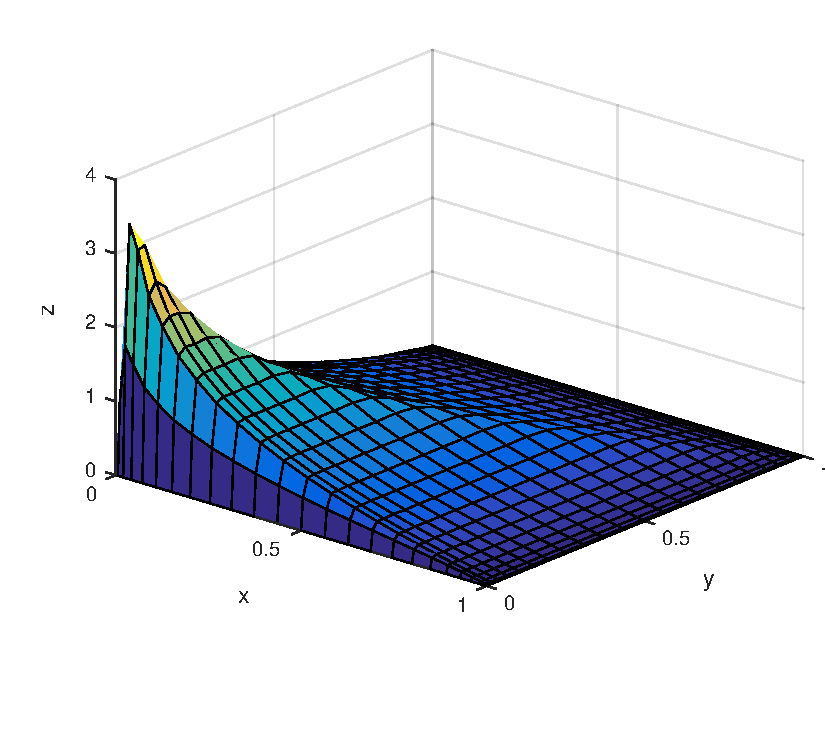
\includegraphics[width=\textwidth]{Figures/SpecLS_difftrans_aNeg.pdf}
  \end{subfigure}
          %(or a blank line to force the subfigure onto a new line)
  \vspace{-0.1\baselineskip}
	\caption{Surf plot of the numerical solution of the diffusion transport problem solved by Galerkin spectral methods to the left and least-squares to the right, $\mu = 10^{-4},N=25,b = 1, \mathbf{b} = -[x,y]$.}
  \label{fig:SurfDiffTransNeg}
\end{figure}
%
Least-squares methods is known to be very stable, and in figure\eref{fig:SurfDiffTransNeg} we see that LS provides a slightly smoother solution than Galerkin. At the same time the peak is a little bit lower, indicating that least-squares has a tendency to even out high gradients.  
%
\begin{figure}[h]
  \centering
  \begin{subfigure}[b]{0.48\textwidth}
	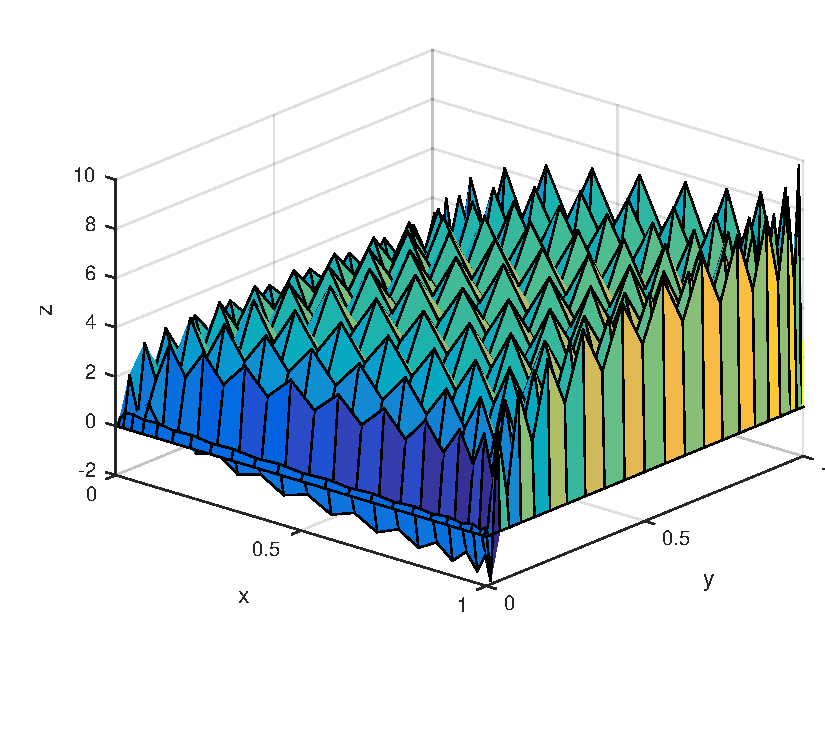
\includegraphics[width=\textwidth]{Figures/Spec_difftrans_aPos.pdf}
  \end{subfigure}%
  \quad
  %\begin{subfigure}[b]{0.48\textwidth}
	%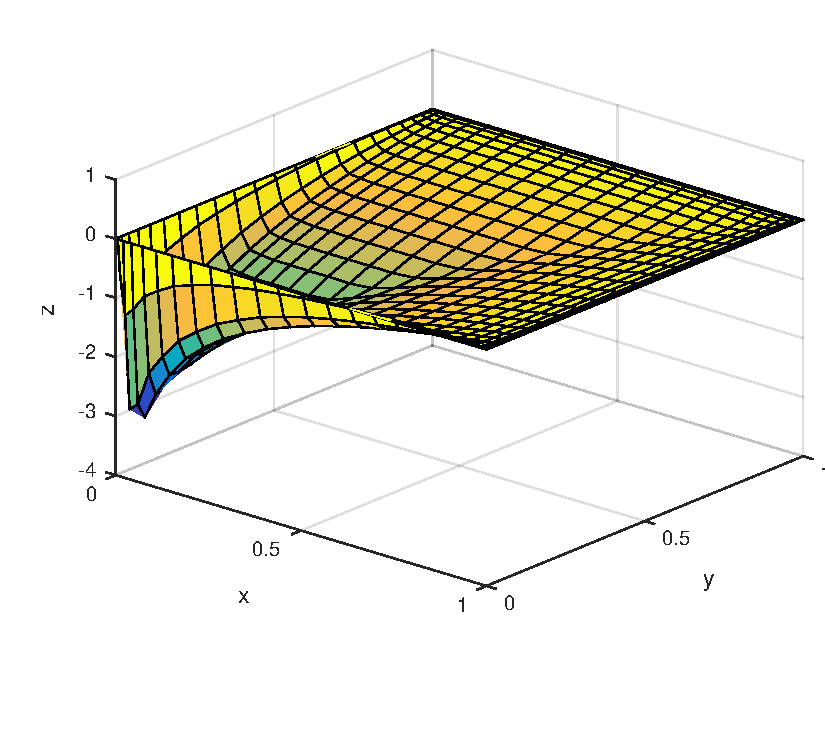
\includegraphics[width=\textwidth]{Figures/SpecLS_difftrans_aPos.pdf}
  %\end{subfigure}
  \begin{subfigure}[b]{0.48\textwidth}
	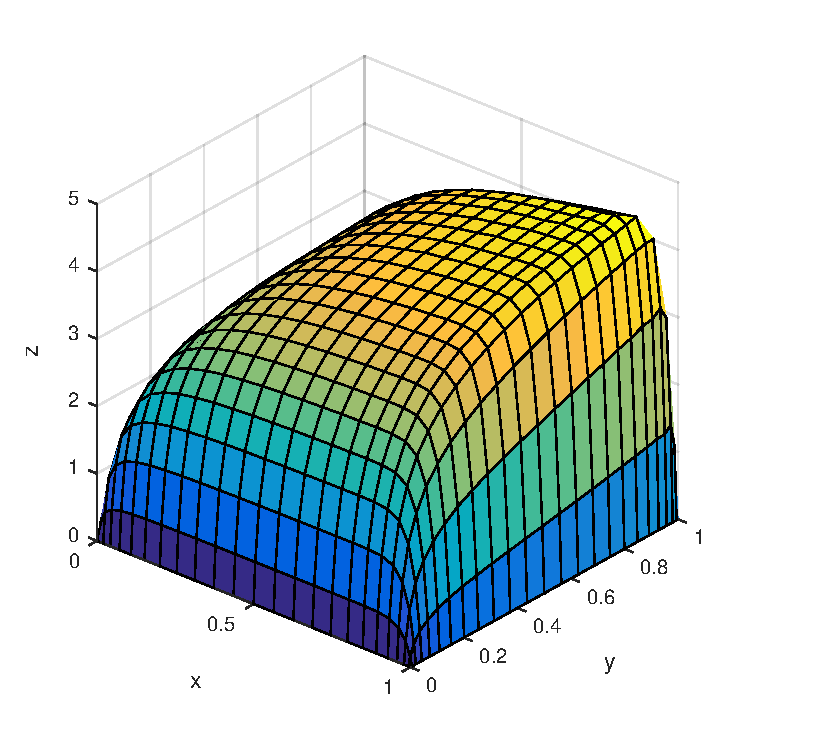
\includegraphics[width=\textwidth]{Figures/SpecGLS_difftrans_aPos.pdf}
  \end{subfigure}
          %(or a blank line to force the subfigure onto a new line)
  \vspace{-0.1\baselineskip}
  \caption{Surf plot of the numerical solution obtained from spectral methods of the diffusion transport problem solved by Galerkin to the left and with a combined GLS method to the right, with smoothing factor $\delta = 0.05$, both plots use the same parameters $\mu = 10^{-4}, N=25,b = 1,\mathbf{b} = [x,y]$.}
  \label{fig:SurfDiffTransPositive}
\end{figure}
%

By using the stability abilities of least-squares and creating the bilinear form as explained in chapter \ref{chap:newTheory} we obtain the results in figure\eref{fig:SurfDiffTransPositive} and figure\eref{fig:SurfDiffTransPositiveFEM}. The smoothing provided by least-squares is indisputable. Note that this is a consistent method, meaning that it does not add a viscous term dependent on the step-length and therefore conserves the convergence rate. 

It works for well for spectral basis functions and the combined GLS bilinear form is easily constructed from the two separate forms. Notice that although the finite element basis functions used in\eref{fig:SurfDiffTransPositiveFEM} are not consistent with the theory the smoothing effect is not that bad.  
%
\begin{figure}[h]
  \centering
  \begin{subfigure}[b]{0.48\textwidth}
	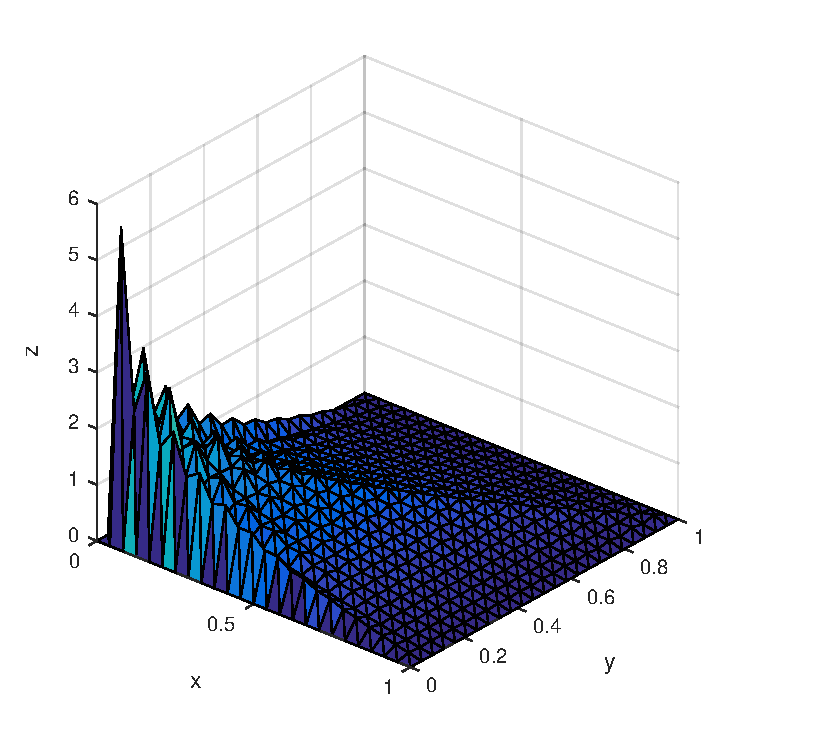
\includegraphics[width=\textwidth]{Figures/FEM_difftrans_aNeg.pdf}
  \end{subfigure}%
  \quad
  %\begin{subfigure}[b]{0.48\textwidth}
	%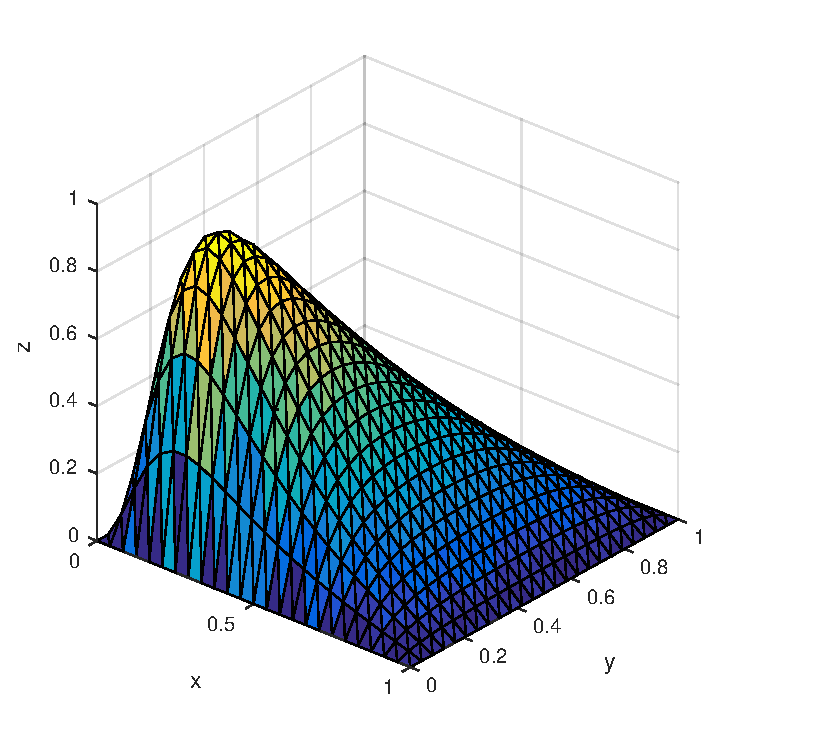
\includegraphics[width=\textwidth]{Figures/LSFEM_difftrans_aNeg.pdf}
  %\end{subfigure}
  \begin{subfigure}[b]{0.48\textwidth}
	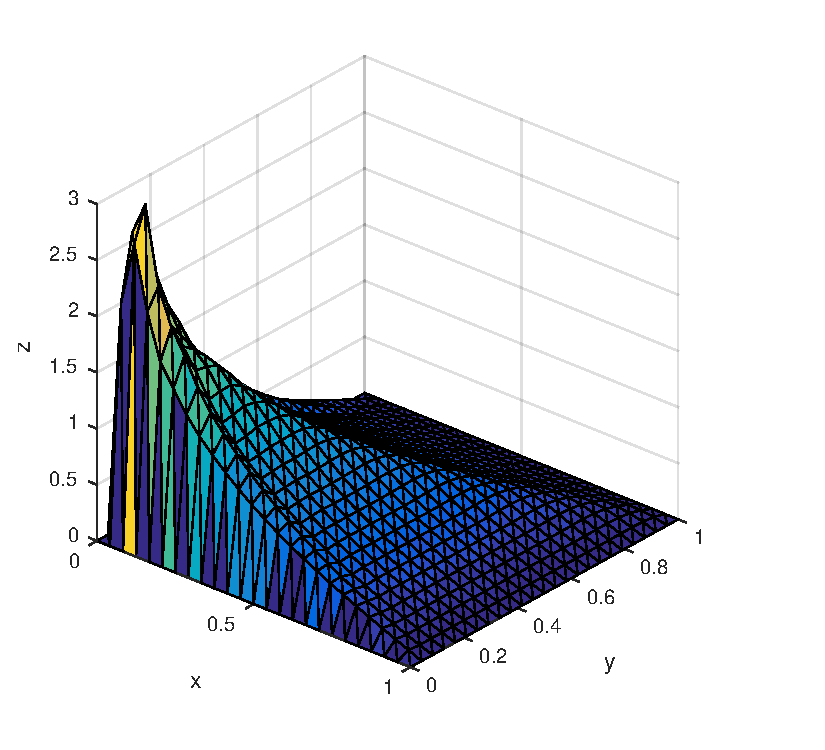
\includegraphics[width=\textwidth]{Figures/GLSFEM_difftrans_aNeg.pdf}
  \end{subfigure}
          %(or a blank line to force the subfigure onto a new line)
  \vspace{-0.1\baselineskip}
	\caption{Surf plot of the numerical solution of the diffusion transport problem solved by Galerkin FEM to the left and the combined GLS method to the right, with smoothing factor $\delta = 0.05$, both plots use the same parameters, $\mu = 10^{-4},N=25,b = 1,\mathbf{b} = -[x,y]$.}
  \label{fig:SurfDiffTransPositiveFEM}
\end{figure}
%
\subsection{Nonlinear results}
The nonlinear equation is constructed by making a minor change in our $\mathbf{b}$-vector, explicitly the vector field is assumed to be on the form $\mathbf{b}=[b_1(x)u,b_2(y)u]$. A test case is constructed in the same way as for the previous problems and the Jacobian is constructed in an analytical and a numerical fashion, the results are shown in figure \ref{fig:convergenceNonlinear}. For the least-squares method the Jacobian is approximated in order to save calculation time, hence we have a quasi-newton method and quadratic convergence is not achieved. Note also that the error from LS converges to a higher value in the same way as it did for the linear problems. 
%
\begin{figure}[h]
  \centering
  \begin{subfigure}[b]{0.48\textwidth}
	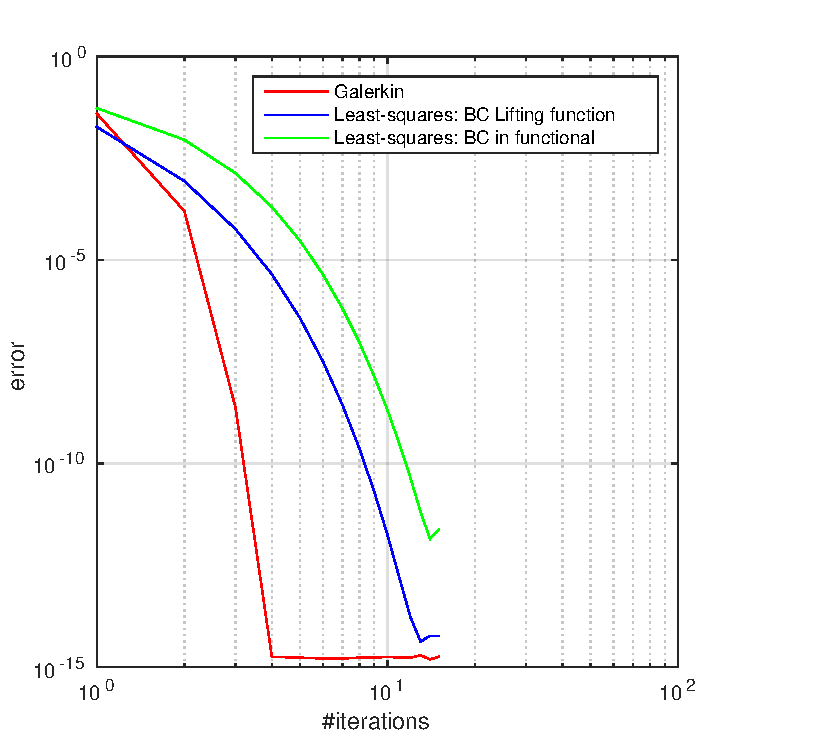
\includegraphics[width=\textwidth]{Figures/Spec_Nonlin_Convergence_Jnum.pdf}
  \end{subfigure}%
  \quad
  \begin{subfigure}[b]{0.48\textwidth}
	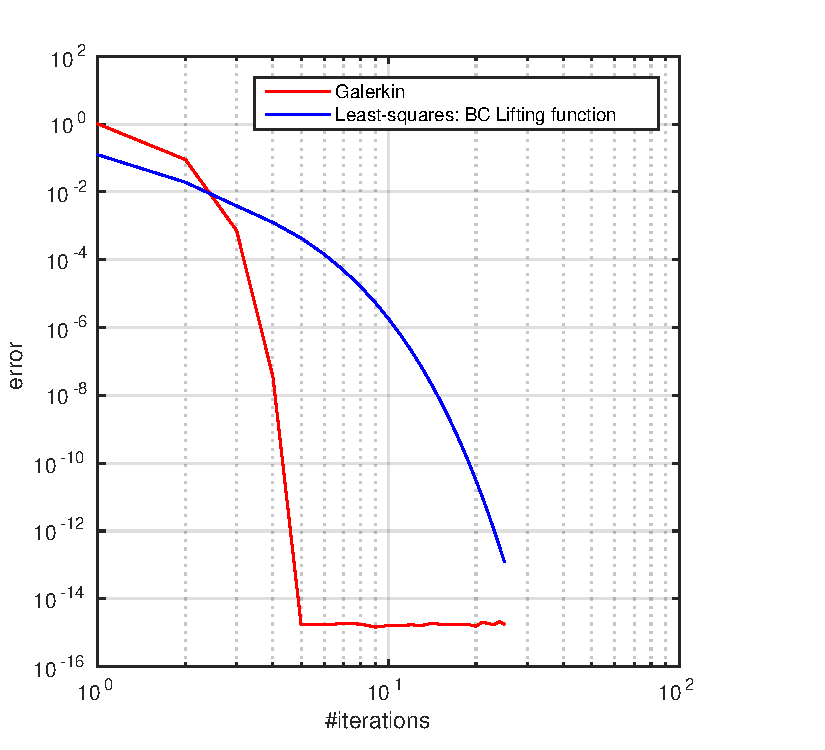
\includegraphics[width=\textwidth]{Figures/Spec_Nonlin_Convergence.pdf}
  \end{subfigure}%
  \vspace{-0.1\baselineskip}
	\caption{Convergence plot of the numerical solution of the nonlinear diffusion transport equation solved by spectral methods, In the figure to the left a numerical Jacobian has been calculated and in the figure to the right the analytical one is used. $\mu = 1,N=15,\mathbf{b} = -[x^2,y^2]$.}
  \label{fig:convergenceNonlinear}
\end{figure}
%
